\section{The certificate under pressure}
\label{sec:pressure}

The experiment is simple to state: a 7B generator writes 64 candidates per problem, each judge configuration picks its favorite, and we check what happened.
Two pre-registered estimands separate deception from damage.
The \emph{excess hack gap} measures scoreboard inflation relative to true quality, in baseline standard deviations over a within-oracle-stratum permutation null (judge scores permuted among samples with the same correctness).
\emph{Oracle regret} measures accuracy left on the table against best-possible selection.
Selection and reporting use different rubric paraphrases, canceling winner's curse.
Item pools are 105 \textsc{MATH-500} and 68 \textsc{MBPP+} items on which the generator sometimes but not always succeeds (pool pass rate in $[0.2, 0.8]$); estimators were committed before generation.

\subsection*{RQ3: Does the audit's verdict predict gaming?}

In-domain, yes, and the answer is per estimand.
The registered predictions were categorical: blind ladder judges fail the audit and referenced ones pass; the sabotaged judge is convicted; failed evaluators are gamed.
On inflation, every failed or convicted configuration (minimum $+0.44\sigma$) exceeds every certified one (maximum $+0.38\sigma$), and the sabotaged frontier's excess gap $+0.85$ $[0.70, 1.00]$ is disjoint from the honest frontier's $+0.38$ $[0.28, 0.51]$.
On regret, every failed blind configuration (minimum $0.324$) exceeds every certified one (maximum $0.117$), but the sabotaged frontier does not separate: its regret $0.133$ is statistically indistinguishable from the honest frontier's $0.117$ (paired difference $+0.014$ $[-0.058, +0.085]$, $n{=}105$ items).
That asymmetry is itself a finding: a style-loaded frontier judge corrupts the scoreboard before it corrupts selection, which is exactly the failure a naive accuracy check cannot see.
We do not claim a pre-frozen numeric threshold; we claim registered categorical verdicts plus the per-estimand separation just stated, with the full 25-configuration accounting in Appendix~\ref{app:confusion}.

\begin{figure}[t]
\centering
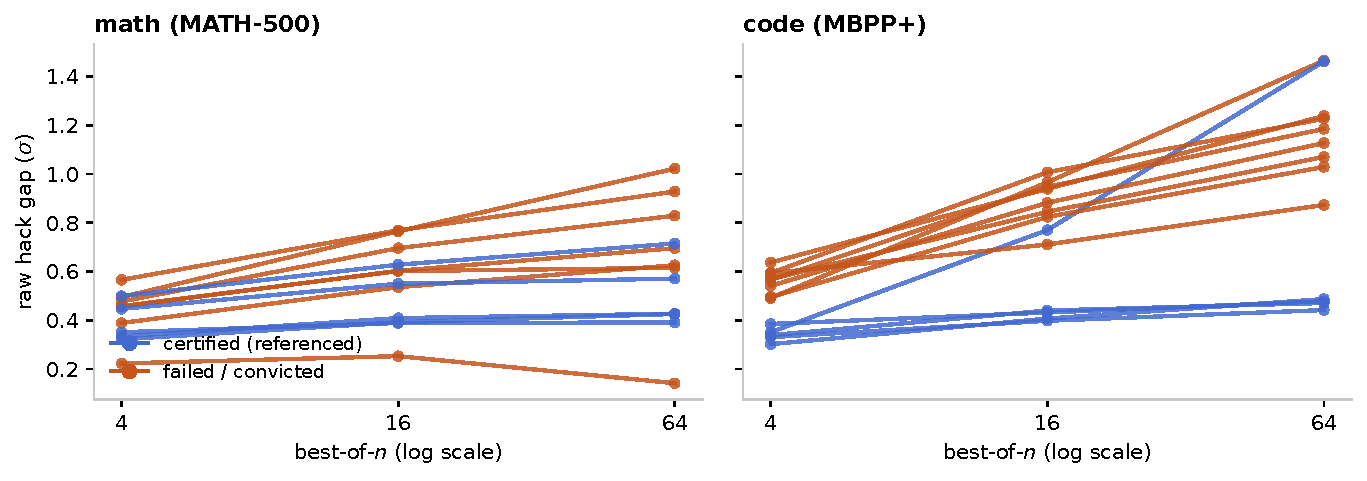
\includegraphics[width=\textwidth]{figures/fig_curves.pdf}
\caption{\textbf{Pressure curves: raw hack gap versus best-of-$n$} for every configuration with existing candidate pools, recomputed at $n = 4, 16, 64$ with the pre-registered estimators.
Blue: certified (referenced) configurations; orange: failed or convicted ones.
\textbf{Takeaway: failed configurations' inflation roughly doubles from $n{=}4$ to $n{=}64$ while certified configurations' rises by less than $0.15\sigma$; the certificate predicts the slope of hacking, not only its endpoint.}}
\label{fig:curves}
\end{figure}

\paragraph{The separation grows with optimization strength.}
Failed configurations steepen and certified ones stay flat (Figure~\ref{fig:curves}).
The blind 3B's code gap runs $+0.64 \to +0.94 \to +1.24$ across $n = 4, 16, 64$, and the blind 7B's $+0.57 \to +0.95 \to +1.19$; the referenced 3B runs $+0.33 \to +0.40 \to +0.44$ and the referenced frontier $+0.39 \to +0.43 \to +0.48$.

\paragraph{Cross-domain transfer, and an in-domain audit with a mechanical target axis.}
The audit generalizes beyond human labels wherever the target axis has an oracle, and code supplies one: executed tests.
We audited every code configuration by the within-item correlation of its scores with test outcomes, with no human labels involved.
The measured rows explain the one extrapolation miss directly: the 1.5B judge's reference adds nothing to its target-axis validity on code ($+0.15$ blind, $+0.16$ referenced), which is the capability gate measured rather than inferred, and that configuration is gamed as badly as its blind twin (Figure~\ref{fig:gate}).
The frontier tier separates cleanly ($+0.52$ blind, $+0.62$ referenced), and sabotage measurably degrades target validity even against a mechanical target ($+0.62 \to +0.42$).
One honest nuance: the 3B judge shows equal target validity blind and referenced ($+0.10$) yet resists inflation only when referenced, so the mechanical-target audit predicts damage well and inflation resistance only through the reference protocol; the human-label axes remain necessary for the deception side.
Operationally: a judge certified on one domain is not thereby certified on another; run the audit, with whatever target oracle the domain offers, where the judge will be used.

\begin{figure}[t]
\centering
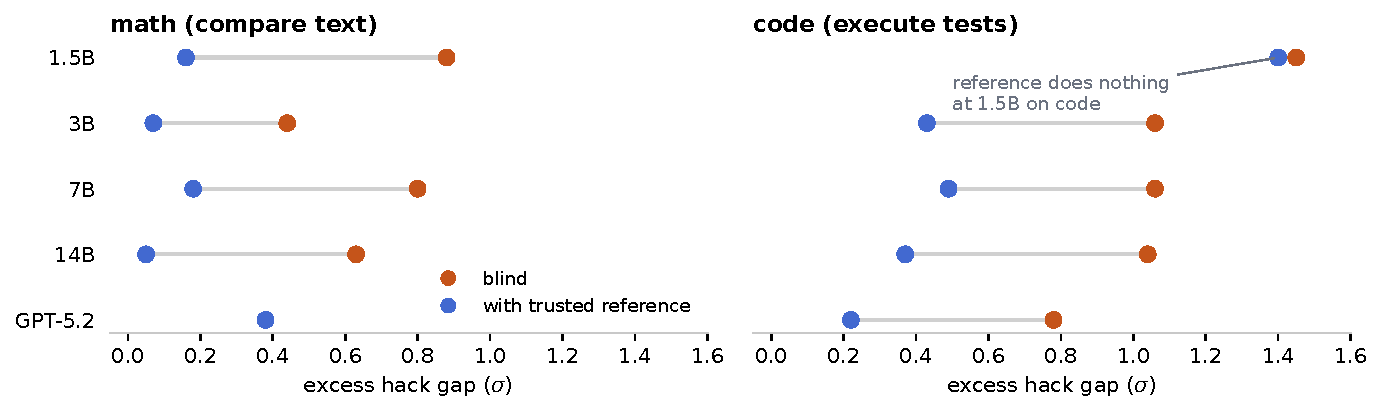
\includegraphics[width=0.9\textwidth]{figures/fig_gate.pdf}
\caption{\textbf{The capability gate.}
Excess hack gap at $n{=}64$ without (orange) and with (blue) a trusted reference, by judge scale and domain.
\textbf{Takeaway: the reference collapses inflation at every scale on math, where using it means comparing text, and only at 3B and above on code, where using it means executing tests.}}
\label{fig:gate}
\end{figure}

\paragraph{Two failure modes, and capability trades one for the other.}
Across the sabotage arms, damage falls and self-inflation rises with judge capability.
The sabotaged 7B damages without inflating (regret $0.400$, gap $+0.13$, not significant); sabotaged GPT-5.2 inflates without measurable damage (gap $+0.85$; regret $0.133$, indistinguishable from the honest frontier's $0.117$).
A blind cross-family panel confirms the channel: sabotage-selected solutions are more styled ($+0.27$ $[0.10, 0.44]$) with no detectable soundness loss.
The frontier mode, deceiving the metric while selecting well, is the one that menaces training.

\paragraph{Granularity beats scale once a reference is in hand.}
The referenced 1.5B outselects the frontier on math because the frontier's 0--10 scale ties $78\%$ of items at the top and random tie-breaks admit wrong answers, while the small judge's continuous expected scores stay sharp.
A registered ablation separates two kinds of granularity.
Re-eliciting the frontier judge on a 0--100 integer scale cuts its regret from $0.117$ to $0.069$ and its gap from $+0.38$ to $+0.27$, confirming the registered prediction, yet top-ties rise to $90\%$ and the frontier still does not approach the small judge's $0.010$.
Elicited granularity helps; distributional granularity, reading the expectation over score-token probabilities, helps more, and only judges that expose token probabilities offer it fully.
